\documentclass[fleqn,10pt,aspectratio=169,dvipsnames]{beamer}
\usetheme[
%%% options passed to the outer theme
%    hidetitle,           % hide the (short) title in the sidebar
%    hideauthor,          % hide the (short) author in the sidebar
%    hideinstitute,       % hide the (short) institute in the bottom of the sidebar
%    shownavsym,          % show the navigation symbols
%    width=2cm,           % width of the sidebar (default is 2 cm)
%    hideothersubsections,% hide all subsections but the subsections in the current section
%    hideallsubsections,  % hide all subsections
    right%left               % right of left position of sidebar (default is right)
%%% options passed to the color theme
%    lightheaderbg,       % use a light header background
  ]{AAUsidebar}

%\definecolor{myBlue}{RGB}{52,52,154}

% If you want to change the colors of the various elements in the theme, edit and uncomment the following lines
% Change the bar and sidebar colors:
%\setbeamercolor{AAUsidebar}{fg=myBlue}
%\setbeamercolor{sidebar}{bg=red!20}
% Change the color of the structural elements:
%\setbeamercolor{structure}{fg=red}
% Change the frame title text color:
%\setbeamercolor{frametitle}{fg=blue}
% Change the normal text color background:
%\setbeamercolor{normal text}{bg=gray!10}
% ... and you can of course change a lot more - see the beamer user manual.

\setlength{\mathindent}{0cm}
\usepackage{xcolor}
\usepackage{color}

% A command to highlight stuff
% \highlight[<colour>]{<stuff>}
\newcommand{\highlight}[2][yellow]{\mathchoice%
	{\colorbox{#1}{$\displaystyle#2$}}%
	{\colorbox{#1}{$\textstyle#2$}}%
	{\colorbox{#1}{$\scriptstyle#2$}}%
	{\colorbox{#1}{$\scriptscriptstyle#2$}}}%

% Define colors
\definecolor{coolBlue}{RGB}{33, 26, 200}
\definecolor{coolRed}{RGB}{200, 42, 42}

% A command to higlight plus name stuff
\definecolor{blueEQ}{RGB}{193, 49, 0}
\definecolor{myGray}{RGB}{84,97,110}
\newlength{\overwritelength}
\newlength{\minimumoverwritelength}
\setlength{\minimumoverwritelength}{0.1cm}
\newcommand{\overwrite}[3][red]{%
	\settowidth{\overwritelength}{$#2$}%
	\ifdim\overwritelength<\minimumoverwritelength%
	\setlength{\overwritelength}{\minimumoverwritelength}\fi%
	\stackrel
	{%
		\begin{minipage}{\overwritelength}%
			\color{#1!40}\centering\tiny #3\\%
			\rule{1pt}{3pt}%
		\end{minipage}}
	{\colorbox{#1!40}{\color{myGray}$\displaystyle#2$}}}

% Trying some videos
\usepackage{multimedia}

%\usepackage[utf8, latin1]{inputenc}
\usepackage[T1]{fontenc}
%\usepackage{fouriernc}

\usepackage[spanish]{babel}
% Or whatever. Note that the encoding and the font should match. If T1
% does not look nice, try deleting the line with the fontenc.
% No indent emunerate
\usepackage{enumitem}
\usepackage{multicol}
\usepackage{wasysym}
%\usepackage{mathpazo}
%\renewcommand\rmdefault{hpv}
%\usepackage{avant}
\usepackage{fontspec}
\usepackage{ragged2e}
\usepackage{color}
\usepackage[customcolors]{hf-tikz}
\usepackage[skins,theorems]{tcolorbox}
\usepackage{mathrsfs,amsmath}
\usepackage{graphicx} 
\usepackage{animate}
\usepackage{multido}
\usepackage{xmpmulti}
%\usepackage{media9}
\usepackage{multimedia}
\usetikzlibrary{positioning, arrows}

\newcommand\scalemath[2]{\scalebox{#1}{\mbox{\ensuremath{\displaystyle #2}}}}
%\usepackage{vwcol} 
%\usepackage{amssymb}
%\tcbset{highlight math style={enhanced, colframe=red,colback=white,arc=0.5pt,boxrule=0.5pt}}

\setmainfont[
Extension=.otf,
UprightFont= *-regular,
BoldFont=*-bold,
ItalicFont=*-italic,
BoldItalicFont=*-bolditalic,
]{texgyreheros}

% Change the font style \rmfamily \normalfont \sffamily
%\renewcommand*\rmdefault{cmss}
%\renewcommand{\familydefault}{\sfdefault}
%\renewcommand{\familydefault}{\rmdefault}

%\usepackage{mathrsfs}
\usefonttheme{professionalfonts}
%\usefonttheme[onlymath]{serif}
%\renewcommand\sfdefault{cmbr}
\usepackage[small,OT1,euler-digits]{eulervm}

% colored hyperlinks
\newcommand{\chref}[2]{%
  \href{#1}{{\usebeamercolor[bg]{AAUsidebar}#2}}%
}


\newcommand\blfootnote[1]{%
	\begingroup
	\renewcommand\thefootnote{}\footnote{#1}%
	\addtocounter{footnote}{-1}%
	\endgroup
}

% Color box
\usepackage{tcolorbox}

% Commands
\newcommand{\invi}{\textit{in vivo}\ }
\newcommand{\exvi}{\textit{ex vivo}\ }

\usepackage{mathtools}
% et al
\newcommand{\etal}{\textit{et al.}\ }
% Subtitle sze
\setbeamerfont{framesubtitle}{size=\normalsize}
% Num sections in TOC
\setbeamertemplate{section in toc}[sections numbered]

\title[CAO en OCT de fase inestable]{\vspace*{\baselineskip} \LARGE Óptica adaptativa computacional en tomografía de coherencia sin estabilidad de fase}

\subtitle{\vspace*{.5\baselineskip}\emph{\bf Trabajo de grado I \\ Maestría en Física Aplicada }\vspace*{-.5\baselineskip}} % could also be a conference name


\newif\ifplacelogo % create a new conditional
\placelogotrue % set it to true

\author[Sebastián Ruiz \vspace*{-1.5\baselineskip}]{\bf 
	\vspace*{-2\baselineskip}Sebastián Ruiz Lopera  \vspace*{\baselineskip}\\
	{\small Asesor: Ph.D. René Restrepo Gómez} \\ Área de Instrumentación Óptica Espacial - INTA \vspace*{.5\baselineskip} \\ {\small Co-asesor: Ph.D. Néstor Uribe Paratarroyo} \\ Wellman Center for Photomedicine - MGH - HMS  \vspace*{\baselineskip}\\
	{\footnotesize Escuela de Ciencias \\ Grupo de Óptica Aplicada} \\
	{\footnotesize{26 de febrero de 2020}}\vspace*{-1.5\baselineskip}
}
% - Give the names in the same order as they appear in the paper.
% - Use the \inst{?} command only if the authors have different
%   affiliation. See the beamer manual for an example

%\institute[]{Maestría en Física Aplicada\\Departamento de Ciencias Físicas\\Escuela de Ciencias}

%\date{1 de febrero de 2018} % Nota : Cambiar la fecha
\date{ }

% specify a logo on the titlepage (you can specify additional logos an include them in 
% institute command below
%\pgfdeclareimage[height=1.8cm]{titlepagelogo}{AAUgraphics/aau_logo_new_circle.pdf} % placed on the title page

\pgfdeclareimage[height=1.3cm]{titlepagelogo}{AAUgraphics/logo_eafit_vig_minedu} % placed on the title page

%\pgfdeclareimage[height=1.5cm]{titlepagelogo2}{graphics/aau_logo_new} % placed on the title page
\titlegraphic{% is placed on the bottom of the title page
	\vspace*{-.5\baselineskip}
  \pgfuseimage{titlepagelogo}
%  \hspace{1cm}\pgfuseimage{titlepagelogo2}
}


\begin{document}
% the titlepage
{\aauwavesbg%
\begin{frame}[plain,noframenumbering] % the plain option removes the sidebar and header from the title page
\titlepage
\end{frame}}

%%%%%%%%%%%%%%%%%%%%%%%%%%%   Contenido   %%%%%%%%%%%%%%%%%%%%%%%%%%%%
\begin{comment}
\begin{frame}{Contenido}{}
\large
	\begin{multicols}{2}
\tableofcontents
	\end{multicols}
\end{frame}
\end{comment}

%%%%%%%%%%%%%%%%%%%%%%%%%%%   Introducción OCT  %%%%%%%%%%%%%%%%%%%%%%%%%%%%

\section{Introducción}

\begin{frame}[c]{Introducción}
\small
\textbf{OCT es susceptible a aberraciones ópticas:} \\
	\begin{itemize}
\item Propias del sistema óptico,
\item Inducidas por la muestra (e.g. imagen retinal). \\
	\end{itemize}

	\begin{centering}
		\begin{columns}
			\begin{column}{\textwidth}
\hspace*{0\baselineskip}
\includegraphics[width=.47\textwidth]{../Figuras/Confocal_gating.png}
\hspace*{.5\baselineskip}
\onslide<2->{\includegraphics[width=.47\textwidth]{../Figuras/Human_photoreceptos.png}}
			\end{column}
		\end{columns}
\vspace{\baselineskip}
\onslide<3>{
{\color{coolRed}Compromiso} entre resolución y profundidad de campo. \\
Las aberraciones {\color{coolRed}afectan} la resolución efectiva del sistema. \\
}
	\end{centering}

\blfootnote{\tiny{W. Drexler \etal Optical Coherence Tomography: Technology and Applications. \emph{Springer,} 2015.}}
\blfootnote{\tiny{P. Pande \etal Opt Lett, 41(14): 3324-3327, 2016.}}
%\vspace{.75\baselineskip}
\end{frame}

\begin{frame}[t]{Introducción}
La corrección computacional de aberraciones (CAC) es un campo de interés en OCT para evitar o complementar los enfoques basados en \textit{hardware}. CAC opera en el campo complejo con \textbf{modelos analíticos} o \textbf{parámetros derivados de los datos mismos.}
	\begin{center}
		\begin{overprint}
\hspace*{-1\baselineskip}
\onslide<2>\includegraphics[height=.55\textheight]{../Figuras/ProblemStatement_1.png}
\onslide<3>\includegraphics[height=.55\textheight]{../Figuras/ProblemStatement_2.png}
\onslide<4>\includegraphics[height=.55\textheight]{../Figuras/ProblemStatement_3.png}
\onslide<5>\includegraphics[height=.55\textheight]{../Figuras/ProblemStatement_4.png}
		\end{overprint}
	\end{center}
\end{frame}

\begin{frame}[t]{Planteamiento del problema}
	\begin{center}
{\onslide<1-> La \textbf{corrección de aberraciones} es de gran interés para potenciar el desempeño de OCT al obtener imágenes que preservan la información de estructuras finas, así como para extender el DOF en imágenes de alta resolución. \\}

\vspace{\baselineskip}
{\onslide<2->Las \textbf{técnicas computacionales} operan con el {\color{coolBlue}campo complejo}, por lo que requieren \textit{estabilidad de fase}, que {\color{coolRed}solo se obtiene en sistemas con configuraciones especificas, limitando su aplicabilidad.} \\}

\vspace{\baselineskip}		
{\onslide<3-> Se propone desarrollar una {\color{coolBlue}estrategia computacional de corrección de aberraciones ópticas} en tomografía de coherencia óptica que pueda {\color{coolBlue}operar en sistemas sin estabilidad de fase}, ampliando así la aplicabilidad de estas técnicas en sistemas más comunes, {\color{coolBlue}sin configuraciones especificas.} \\}
	\end{center}
\end{frame}

\section{Objetivos}
\subsection{Objetivo general}
\subsection{Objetivos específicos}

\begin{frame}[t]{Objetivos}

{\bf \large Objetivo general}

Corregir aberraciones ópticas en tomografía de coherencia óptica {\color{coolBlue}sin estabilidad de fase} mediante técnicas de {\color{coolBlue}posprocesamiento.} \\
\vspace{\baselineskip}

\onslide<2->{
{\bf \large Objetivos específicos}
}

	\begin{itemize}
    
\item<2-> Establecer el {\color{coolBlue}estado del arte} de la corrección computacional de aberraciones ópticas en tomografía de coherencia óptica.
    
\item<3-> Identificar las {\color{coolBlue}fuentes de inestabilidades de fase} y los {\color{coolBlue}métodos de estabilización de tomogramas} adquiridos mediante tomografía de coherencia óptica.
    
\item<4-> Desarrollar un {\color{coolBlue}método de posprocesamiento} que permita estabilizar la fase y corregir las aberraciones en tomogramas adquiridos sin estabilidad de fase.
    
\item<5-> Evaluar el desempeño del método con {\color{coolBlue}datos experimentales} \invi\ y \exvi\ con sistemas típicos con inestabilidades de fase.
    
\item<6-> Identificar y analizar las posibles {\color{coolBlue}limitaciones del método.}
    
	\end{itemize}

\end{frame}

\begin{frame}[t]{Metodología}
\includegraphics<1>[width=\textwidth]{../Figuras/Metodologia_1.pdf}
\includegraphics<2>[width=\textwidth]{../Figuras/Metodologia_2.pdf}
\includegraphics<3>[width=\textwidth]{../Figuras/Metodologia_3.pdf}
\includegraphics<4>[width=\textwidth]{../Figuras/Metodologia_4.pdf}
\end{frame}


\begin{frame}[t]{Cronograma}
\vspace{-.5\baselineskip}
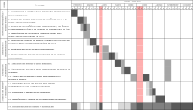
\includegraphics[width=.95\textwidth]{../Figuras/Cronograma.pdf}
\end{frame}

%---------------------------------------------------------------%
%\begin{frame}{Agradecimientos}
%	\begin{itemize}
%		\item Al asesor René Restrepo.
%		\item A los integrantes del grupo: Camilo, Daniel, Carlos, Alejandro, Daniela, Juan José, Elena y a los demás...
%	\end{itemize}
%\end{frame}

{\aauwavesbg%
	\begin{frame}[plain,noframenumbering]
		\finalpage{¡Gracias por su atención! \\ ¿Alguna pregunta?}%\\ Enviarla al correo ccuarta1@eafit.edu.co}
	\end{frame}}

\end{document}
